%----------------------------------------------------------------------------------------
%	INTRODUCTION
%----------------------------------------------------------------------------------------

\section*{RISC-V I/O}

	% Introduction
	Para lidar com dispositivos de entrada/saída, a ISA do RISC-V prevê um esquema de
	\textit{Memory Mapped I/O} (MMIO), ou seja, o RISC-V se utiliza do mesmo espaço de endereçamento
	para endereçar tanto memória quanto dispositivos de entrada e saída. Dessa forma, a
	especificação da ISA não prevê nenhum tipo de instrução especial para controle ou manipulação
	do barramento para realizar I/O, mas sim as mesmas instruções utilizadas para acessar a
	memória são aplicadas para acessar endereços dentro do espaço de endereçamento
	que se referem a dispositivos externos.

	Esse princípio se apoia na ideia de se ter uma ISA que seja simples e que possua instruções
	simples, uma vez que não se tem instruções adicionais para se lidar com operações de entrada
	e saída, apenas aquelas previamente existentes para acesso à memória. Além disso, o esquema
	de entrada e saída mapeado em memória também incorre num design de CPU mais simples e mais
	eficiente, além do fato de que utilizar as instruções regulares de memória para I/O permite
	utilizar qualquer um dos modos de endereçamento suportados pela CPU para endereçar
	esses dispositivos. Além de simplificar a programação, isso também força uma proteção nos
	acessos de dados através do espaço de endereçamento, evitando que \textit{threads} do espaço
	do usuário acessem endereços mapeados para entrada e saída diretamente.


	\subsection*{Memory Mapped I/O (MMIO)}
		A ideia do esquema de MMIO consiste no fato de que cada um dos dispositivos de entrada e
		saída sejam mapeados e associados para um ou mais endereços dentro do espaço de endereçamento do
		sistema. A partir dai, cada um dos dispositivos de I/O passa a monitorar o barramento de
		endereços da CPU, afim de interceptar requisições para qualquer um de seus endereços associados.
		É importante notar que aqui não se fala de reservar um espaço dentro da memória para comunicação
		com o dispositivo, mas sim de mapear os registradores de \textit{hardware} dos dispositivos para dentro
		do espaço de endereçamento do processo.

		Esse mapeamento do espaço de endereçamento fica a cargo do ambiente de execução, e geralmente é
		realizado durante o boot do sistema, sendo feito por algum \textit{firmware} ou por alguma
		\textit{Memory Management Unit} (MMU). No RISC-V, as regiões do espaço de endereçamento podem
		ser mapeadas como: (i) memória, (ii) I/O ou (iii) vazias, que basicamente são regiões de I/O sem
		permissões de acesso. Cada região então possui \textit{Physical Memory Attributes} (PMAs) específicos
		que definem as operações passíveis de serem realizadas sobre aquele intervalo de endereços, sua
		acessibilidade, além de uma série de outras características que tratam da maneira como aquela região
		é tratada, como por exemplo se ela é uma região que é passível de ser otimizada via \textit{cache}
		ou não.

		A respeito das regiões de I/O, elas tipicamente são acessadas através de \textit{uncached loads/stores},
		isto é, é feito um \textit{bypass} na memória \textit{cache} e os dados são buscados diretamente
		dos controladores de dispositivos. Esse fato dos periféricos não poderem ser acessados da mesma
		maneira que a memória principal, passível de ser armazenada na \textit{cache}, se encontra
		nos requisitos de consistência existentes no caso de operações de I/O, além dos possíveis efeitos
		colaterais que são passíveis de acontecer em leituras e escritas de dispositivos de entrada
		e saída. Além disso, regiões de I/O ainda podem especificar quais combinações de permissões de
		acesso são válidas dentro do seu intervalo, além das larguras de dados suportadas pelos dispositivos
		aos quais elas mapeiam.

		No porte do RISC-V no emulador QEMU, o protocolo utilizado para o mapeamento de I/O é o VirtIO, que
		emula dispositivos externos virtuais e visa estabelecer uma API padrão para comunicação com esses
		dispositivos. Voltando ao porte do RISC-V, o QEMU faz o mapeamento desses dispositivos do VirtIO
		a partir do endereço \texttt{0x10001000} até \texttt{0x10008000}, de trás para frente, isto é, se
		tivermos apenas um dispositivo, ele deve estar mapeado para o endereço \texttt{0x10008000}.

		\begin{figure}[bt]
			\begin{commandline}
				\begin{verbatim}
					$info mtree
					...
					memory-region: system
					    0000000000000000-ffffffffffffffff (prio 0, i/o): system
					        ...
					        0000000010001000-00000000100011ff (prio 0, i/o): virtio-mmio
					        0000000010002000-00000000100021ff (prio 0, i/o): virtio-mmio
					        0000000010003000-00000000100031ff (prio 0, i/o): virtio-mmio
					        0000000010004000-00000000100041ff (prio 0, i/o): virtio-mmio
					        0000000010005000-00000000100051ff (prio 0, i/o): virtio-mmio
					        0000000010006000-00000000100061ff (prio 0, i/o): virtio-mmio
					        0000000010007000-00000000100071ff (prio 0, i/o): virtio-mmio
					        0000000010008000-00000000100081ff (prio 0, i/o): virtio-mmio
					        ...
				\end{verbatim}
			\end{commandline}
			\caption{QEMU VirtIO Map.}
		\end{figure}


	\subsection*{Ordenamento de operações I/O}

		% Introdução
		Uma vez que a ISA do RISC-V prevê um esquema de ordenamento relaxado de memória como
		uma forma de otimizar o desempenho desse subsistema, são necessárias formas de se forçar
		algum tipo de ordenamento para o caso de operações que necessariamente tenham que ocorrer
		antes de outras. No caso de I/O, por exemplo, um ordenamento rígido pode ser utilizado
		para melhorar a compatibilidade com códigos legados de drivers de dispositivos, ou ainda
		ser necessário em alguns casos para garantir a corretude de programas em ambientes que
		possuam vários componentes executando operações em paralelo.

		Acessos a regiões de I/O são visíveis para outras \textit{threads}, dispositivos de controle
		de barramento e pelos próprios dispositivos alvo desses acessos. Essas regiões podem tanto
		implementar políticas de ordenamento relaxadas quanto rígidas. Uma região com ordenamento
		relaxado não garante nenhum ordenamento nos acessos a esses dispositivos, à exceção daqueles
		impostos por instruções \texttt{FENCE}, enquanto uma região de I/O com ordenamento
		rígido garante que todos os acessos feitos por uma \textit{thread} àquela região sejam observados
		pelos outros observadores na ordem programada. Assim, cada região de I/O com ordenamento
		rígido especifica um número de canal, que é um mecanismo que garante que ordenamento possa
		ser provido entre diferentes regiões. Por exemplo, o canal 0 especifica ordenamento rígido
		apenas entre uma \textit{thread} e a região especificada, enquanto o canal 1 é usado para prover
		ordenamento global entre todas as regiões de I/O. No entanto, para se ter um controle mais
		fino de quais acessos têm que preceder, sem a necessidade de um ordenamento total, tem-se
		a instrução FENCE, que garante que todas as operações do grupo predecessor sejam vistas
		pelos observadores antes do grupo de operações sucessoras à instrução FENCE.

		\begin{figure}[t]
			\centering
			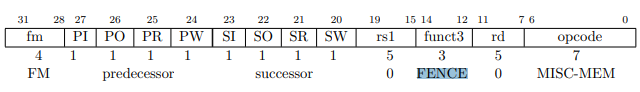
\includegraphics[width=\linewidth]{fence_spec.png}
			\caption{Fence instruction.}
		\end{figure}

		A instrução permite a especificação de qualquer conjunto de \textit{Inputs} (I),
		\textit{Outputs} (O), \textit{Reads} (R) e \textit{Writes} (W) que devam ser
		ordenadas. Essa distinção entre operações de memória (R/W) e de entrada e saída (I/O)
		serve para evitar serialização desnecessária em um \textit{driver} de dispositivo, além
		de permitir outros caminhos que não sejam a memória para controlar coprocessadores ou
		dispositivos de I/O.


%----------------------------------------------------------------------------------------